% Chapter 3 - Results 

\chapter{Numerical experiments} % Main chapter title

\label{chap:results} % For referencing the chapter elsewhere, use \ref{Chapter1} 

\lhead{Chapter 3. \emph{Comparison of methods}} % This is for the header on each page - perhaps a shortened title

%----------------------------------------------------------------------------------------
\section{General results}
Using least squares assures a SPD system which is an important advantage over regular Galerkin. On the downside the matrix obtained from least squares is a lot worse conditioned and complex to create. For second order equations this system is three times as big as if we were to solve it without doing the transformation to a set of hyperbolic equations, which is the most convenient way to use least squares. Comparing the correctness of the solution to the problems
%as done in for example figure~\ref{fig:ConvergencePoisson} shows that the convergence rate is the same as for Galerkin, but with a finite element basis the value of the residual is slightly higher for the least squares method, and for spectral basis functions least squares converge to a higher residual.
reveals that the least squares solution is slightly higher, this effect can be explained by the functional that is minimized. Notice that in the least squares methods you minimize the \textbf{square} of the residual, while with Galerkin you minimize the residual itself. Since the correctness of both methods are restricted by the smoothness of the solution and the number of discrete points LS-methods will minimize the residual squared down to a given precision and hence the residual itself to a slightly higher value. 
%\newpage
%
\subsection{Poisson problem}
The test case is constructed by choosing the loading function and analytical solution as 
\begin{align}
	f(x,y) &=  e^{x}(\pi^2-1)\sin(\pi y)\\
	u(x,y) &=  e^{x}\sin(\pi y) % Analytical solution
	\label{eq:poissonTestCasevariables}
\end{align}
%
The corresponding Poisson equation is then solved by imposing the Dirichlet boundary condition $g$ such that $g(\partial \Omega) = u(\partial \Omega)$.
In figure\eref{fig:ConvergencePoisson} the convergengence in $L^{\infty}$ is plotted. In the finite element case the least squares solution is slightly higher but has the same convergence rate. Using a spectral basis the least squares solution seems to converge slightly faster, but to a higher residual. The condition number as a function of the number of basis functions is plotted in figure\eref{fig:ConditionPoisson}. The finite element comparison indicates that the condition number only differs with a constant. \colorbox{yellow}{Why is the spectral case a order different!!!??}. 
%
\begin{figure}[t]
  \centering
  \begin{subfigure}[b]{0.48\textwidth}
	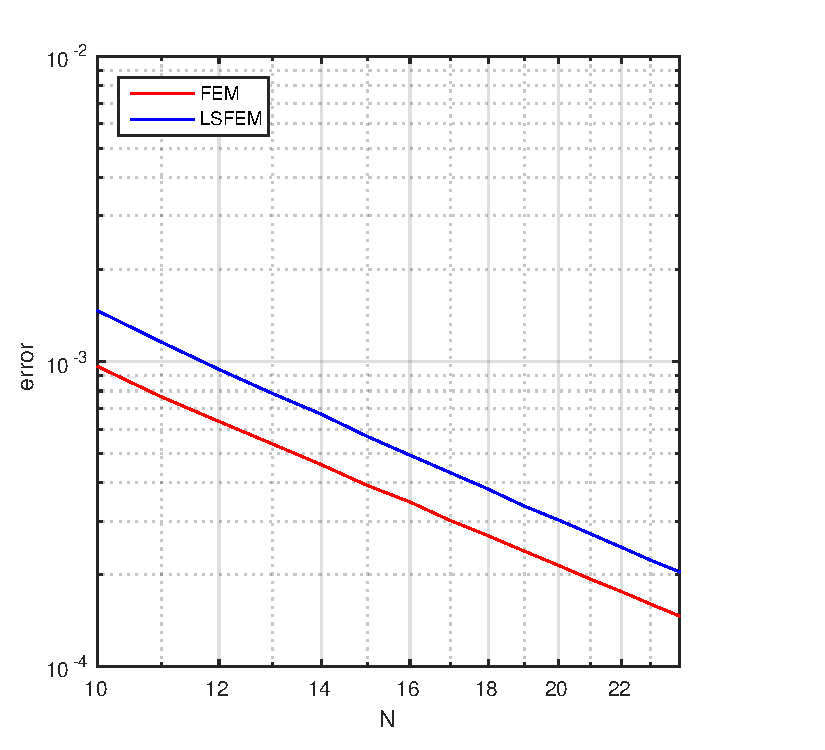
\includegraphics[width=\textwidth]{Figures/errorFEM-LSFEM.pdf}
  \end{subfigure}%
  \quad
  \begin{subfigure}[b]{0.48\textwidth}
	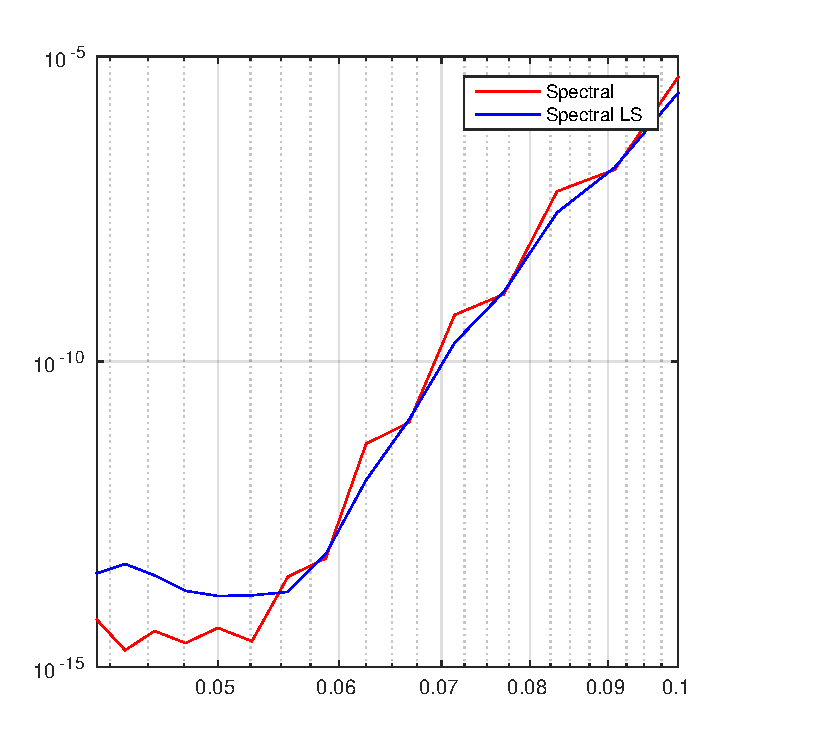
\includegraphics[width=\textwidth]{Figures/errorSpec-SpecLS.pdf}
  \end{subfigure}
          %(or a blank line to force the subfigure onto a new line)
  \vspace{-0.1\baselineskip}
  \caption{Convergence of Galerkin and corresponding least-squares formulation on the Poisson problem.}
  \label{fig:ConvergencePoisson}
\end{figure}
%
\begin{figure}[ht]
  \centering
  \begin{subfigure}[b]{0.48\textwidth}
	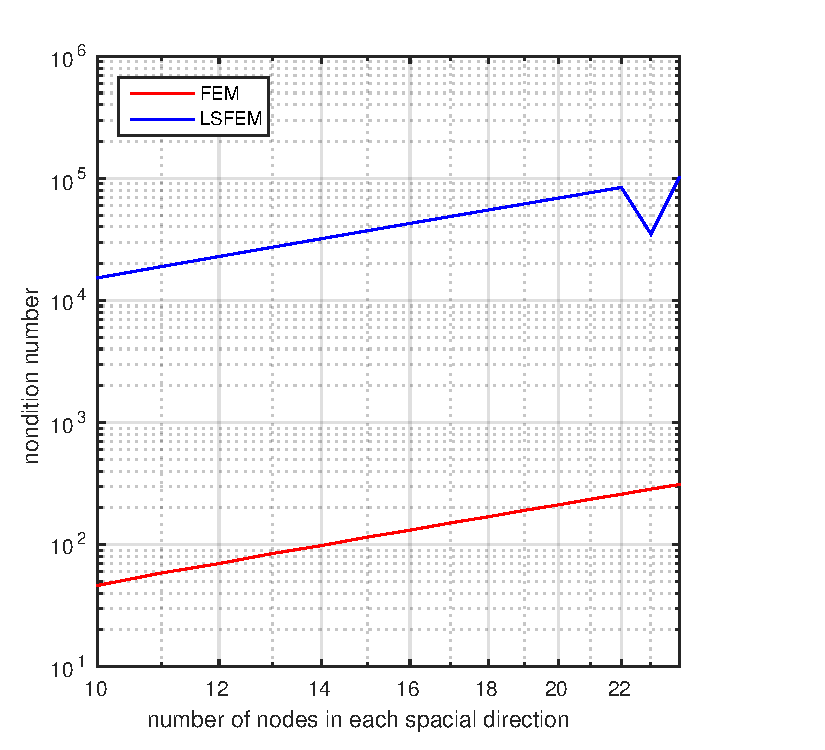
\includegraphics[width=\textwidth]{Figures/condFEM-LSFEM.pdf}
  \end{subfigure}%
  \quad
  \begin{subfigure}[b]{0.48\textwidth}
	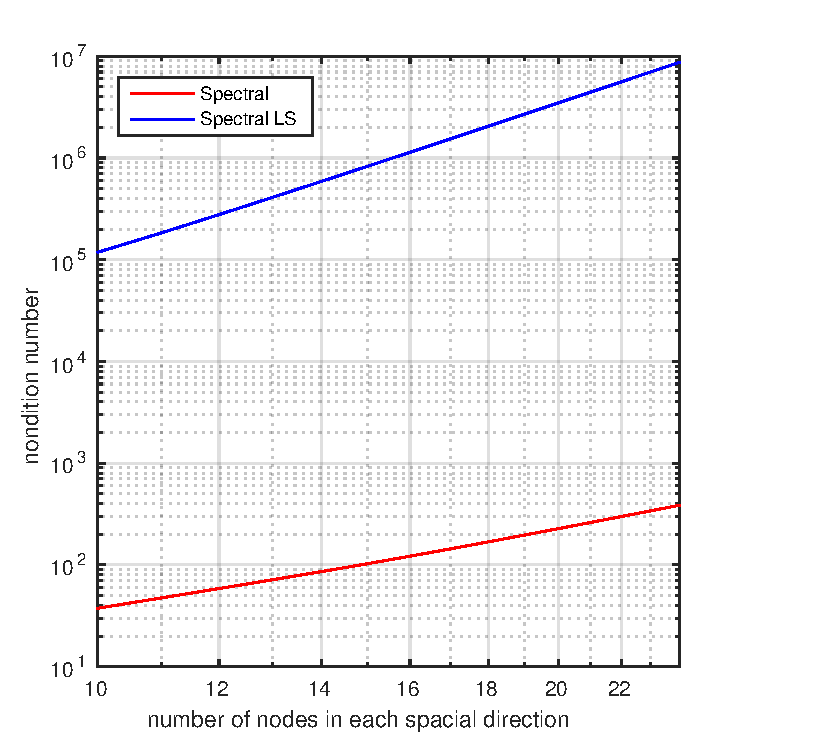
\includegraphics[width=\textwidth]{Figures/condSpec-SpecLS.pdf}
  \end{subfigure}
          %(or a blank line to force the subfigure onto a new line)
  \vspace{-0.1\baselineskip}
  \caption{Condition number of Galerkin and corresponding least-squares formulation on the Poisson problem.}
  \label{fig:ConditionPoisson}
\end{figure}
%
\subsection{Diffusion transport problem}
For this problem I will present results obtained with spectral basis functions. It is also experimented with different ways of implementing the boundary conditions, both Dirichlet and Neumann conditions are implemented using both methods described in section \ref{BC}.
Let us start by letting $\mathbf{b} = [b_1(x),b_2(y)] $ be the normalized vector field in $L^{\infty}$ sence, and  $\mu,b \in \mathbb{R}$ be the scalars used to scale the diffusion and convectional term. The equation analysed is then written as 
\begin{align}
	-\mu \Delta u + b \; (\mathbf{b} \cdot \nabla u) = f .
	\label{eq:difftransForConditionNumberPlotting}
\end{align}
In figure\eref{fig:CondDifftransSpec} the condition number is analysed as a function of the relation between the parameters $\mu,b$. With the steplength/node distance held constant this is proportional to the Peclet number $\mathbb{P}e \sim |b|/\mu$. Notice that along the blue lines $\mu$ is decreasing and $b$ is held constant, while along the red lines $\mu$ is held constant and $b$ is decreasing. The plots reveal that for the least squares case the condition number is significantly more dependent on large $b$ than on small $\mu$. 

The convergence results are presented in figure\eref{fig:ConvergenceDifftransSpec} and the same results as for the Poisson problem are obtained. It is also clear that imposing the boundary conditions as a restriction in our search space is far more efficient than adding them as an extra term to the functional. 

%
\begin{figure}[h!]
  \centering
  \begin{subfigure}[b]{0.48\textwidth}
		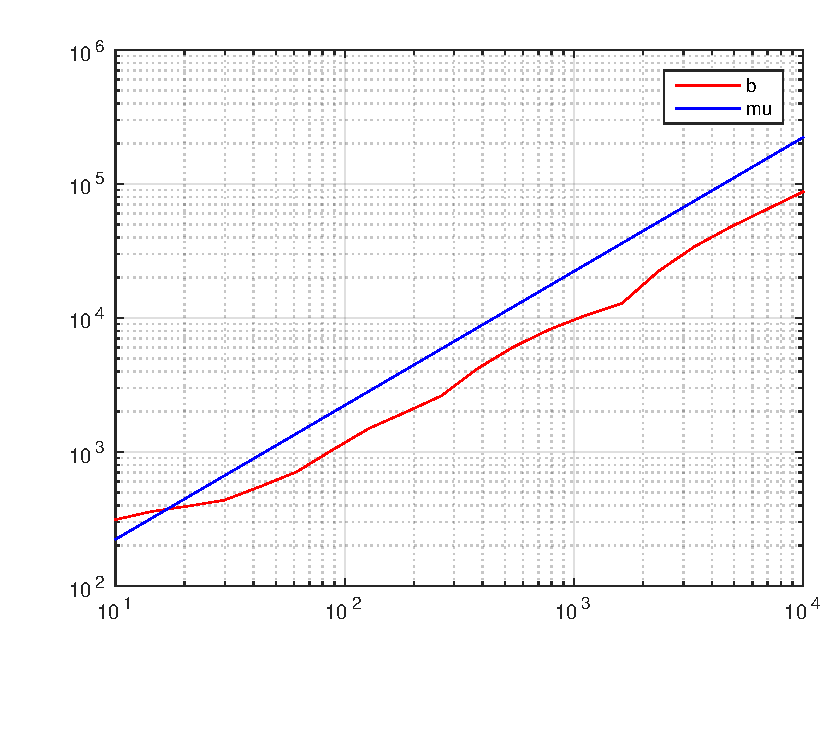
\includegraphics[width=\textwidth]{Figures/Spec_difftrans_ConditionNumber.pdf}
  \end{subfigure}%
  \quad
  \begin{subfigure}[b]{0.48\textwidth}
		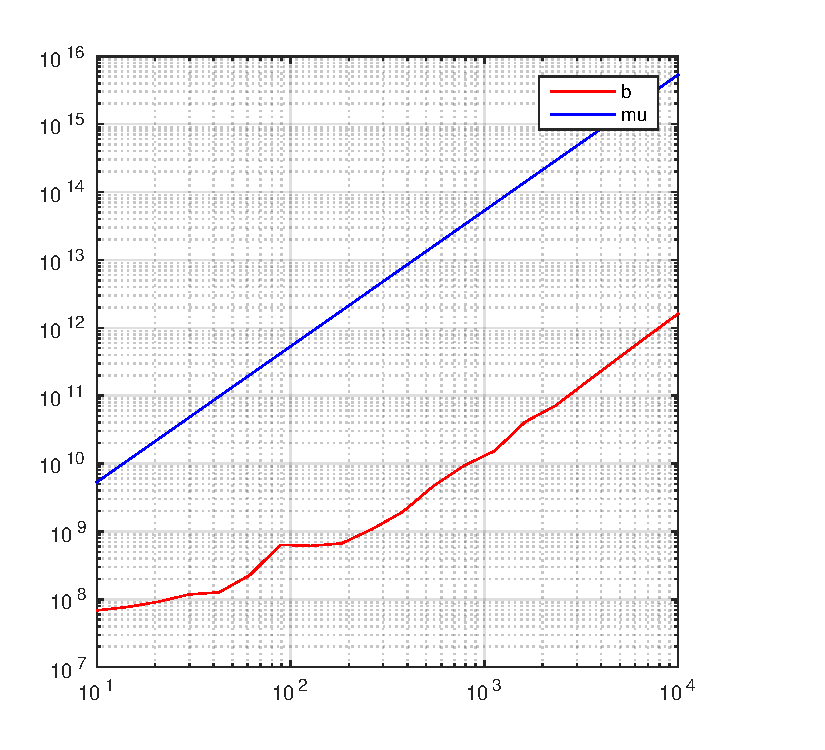
\includegraphics[width=\textwidth]{Figures/Spec-LS_difftrans_ConditionNumber.pdf}
  \end{subfigure}
  \begin{subfigure}[b]{0.48\textwidth}
		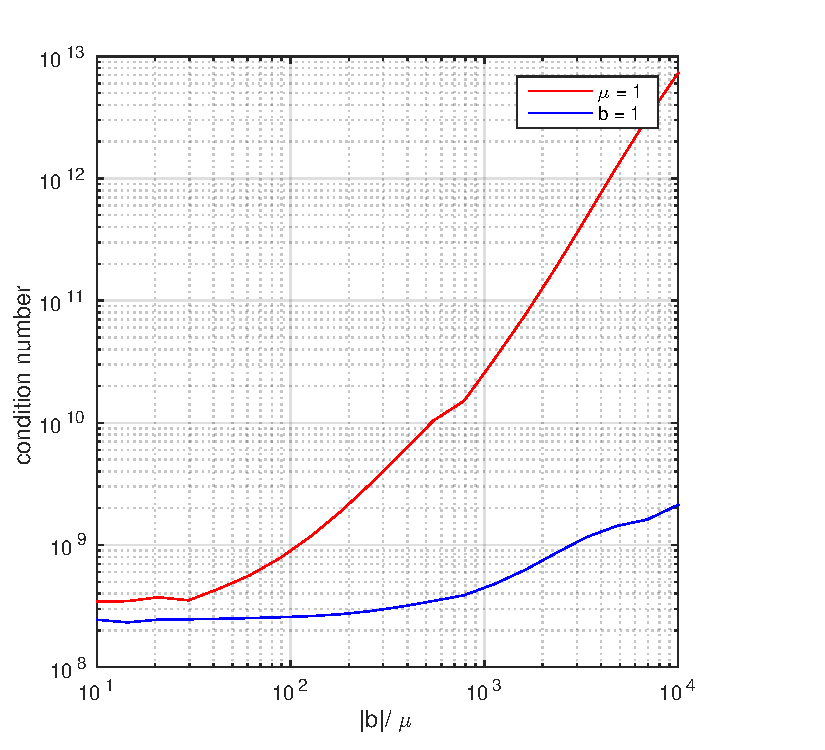
\includegraphics[width=\textwidth]{Figures/Spec-LS_difftrans_ConditionNumber_DirFunc.pdf}
  \end{subfigure}
          %(or a blank line to force the subfigure onto a new line)
  \vspace{-0.1\baselineskip}
	\caption{plot of the condition number as a function of $|b|/\mu \sim \mathbb{P}e$ where $\mathbb{P}e$ is the Peclet number. The parameters $\mu$ and $b$ are varied in turns, $N=20,\mathbf{b} = -[x,y]$. In the upper left plot standard galerkin is used, in the upper right I have implemented a least-squares formulation with boundary conditions implemented directly into the search space. Finally in the lower plot least squares is used with the BC's added in the functional.}
  \label{fig:CondDifftransSpec}
\end{figure}
%
%
\begin{figure}[h!]
  \centering
  \begin{subfigure}[b]{0.48\textwidth}
		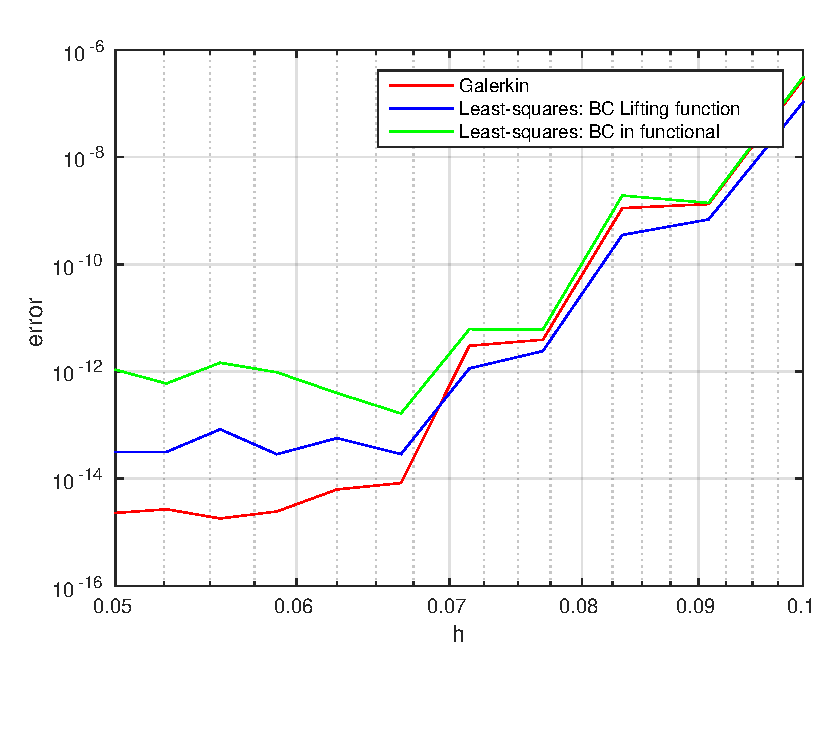
\includegraphics[width=\textwidth]{Figures/Spec_difftrans_Convergence.pdf}
  \end{subfigure}%
  \quad
  \begin{subfigure}[b]{0.48\textwidth}
		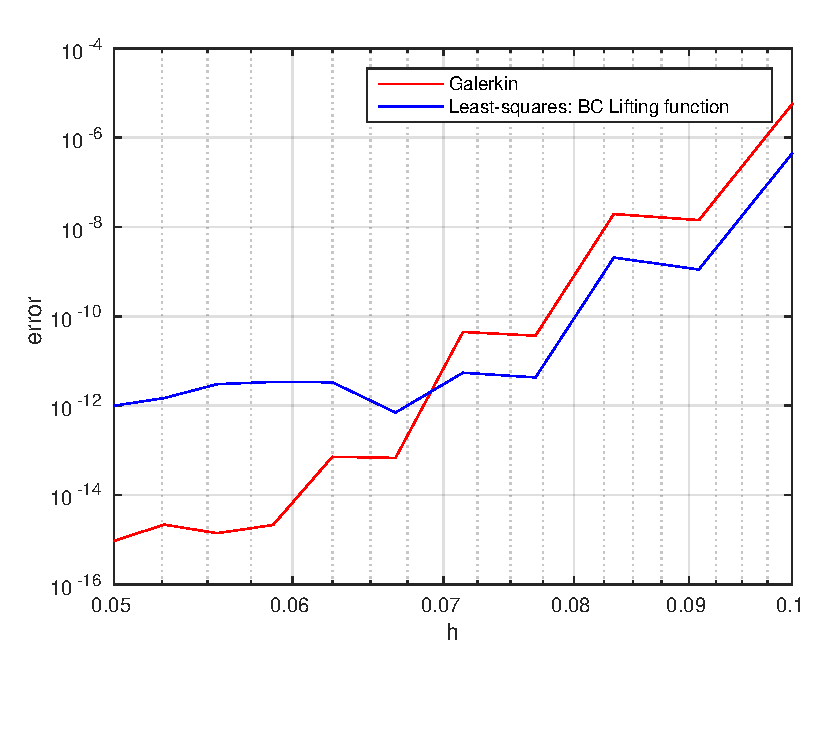
\includegraphics[width=\textwidth]{Figures/Spec_difftrans_Convergence_Neu.pdf}
  \end{subfigure}
          %(or a blank line to force the subfigure onto a new line)
  \vspace{-0.1\baselineskip}
	\caption{convergence plot with pure Dirichlet boundary conditions to the left and Neumann to the right  $\mathbf{b} = -[x,y]$.}
  \label{fig:ConvergenceDifftransSpec}
\end{figure}
%

\subsection{Diffusion transport equation surface plots}
\begin{figure}[h]
  \centering
  \begin{subfigure}[b]{0.48\textwidth}
	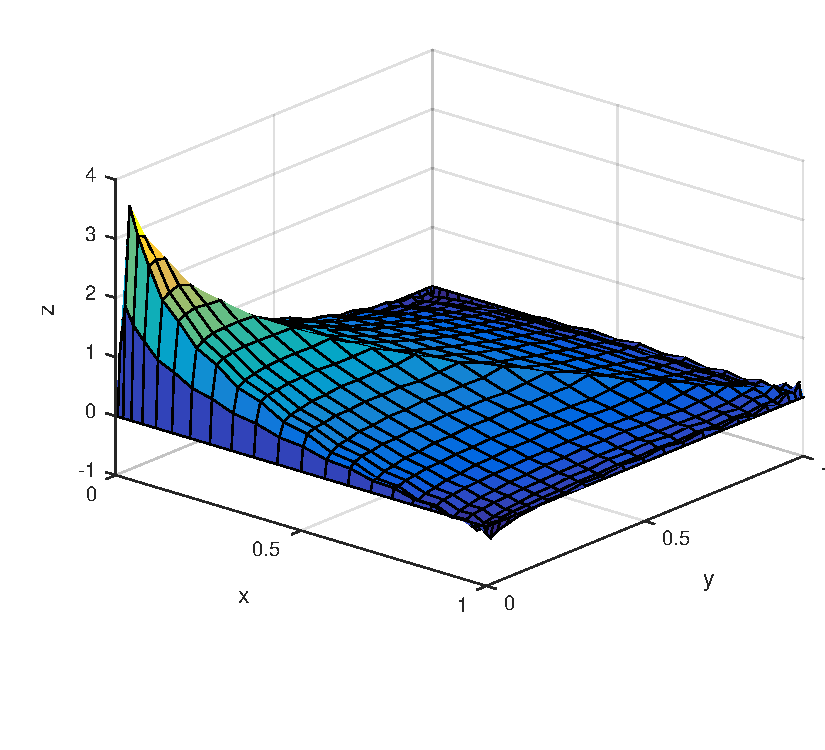
\includegraphics[width=\textwidth]{Figures/Spec_difftrans_aNeg.pdf}
  \end{subfigure}%
  \quad
  \begin{subfigure}[b]{0.48\textwidth}
	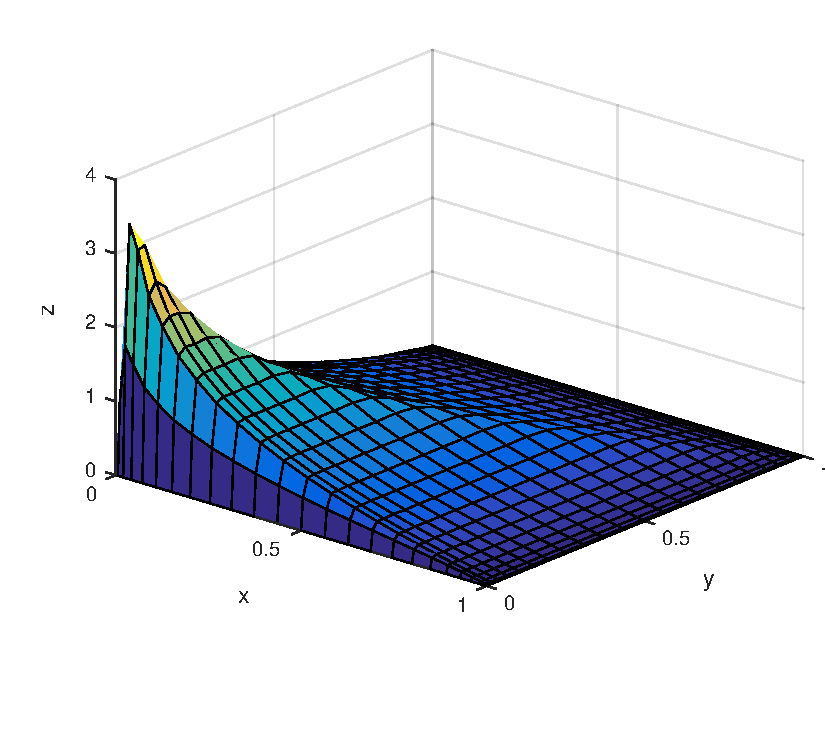
\includegraphics[width=\textwidth]{Figures/SpecLS_difftrans_aNeg.pdf}
  \end{subfigure}
          %(or a blank line to force the subfigure onto a new line)
  \vspace{-0.1\baselineskip}
	\caption{Surf plot of the numerical solution of the diffusion transport problem solved by Galerkin spectral methods to the left and least-squares to the right, $\mu = 10^{-4},N=25,\mathbf{b} = -[x,y]$.}
  \label{fig:SurfDiffTransPositive}
\end{figure}
%
\begin{figure}[h]
  \centering
  \begin{subfigure}[b]{0.48\textwidth}
	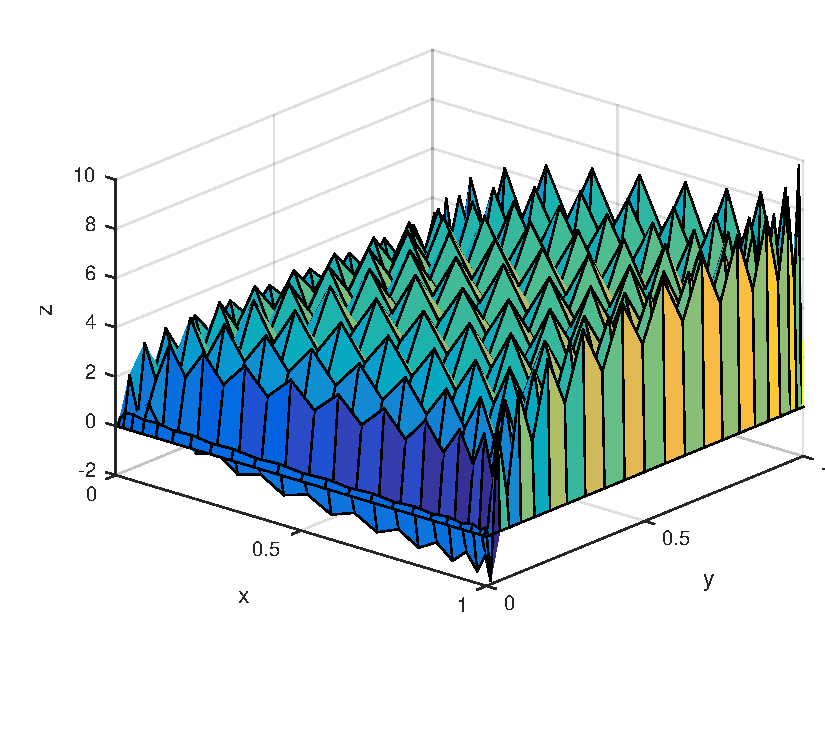
\includegraphics[width=\textwidth]{Figures/Spec_difftrans_aPos.pdf}
  \end{subfigure}%
  \quad
  %\begin{subfigure}[b]{0.48\textwidth}
	%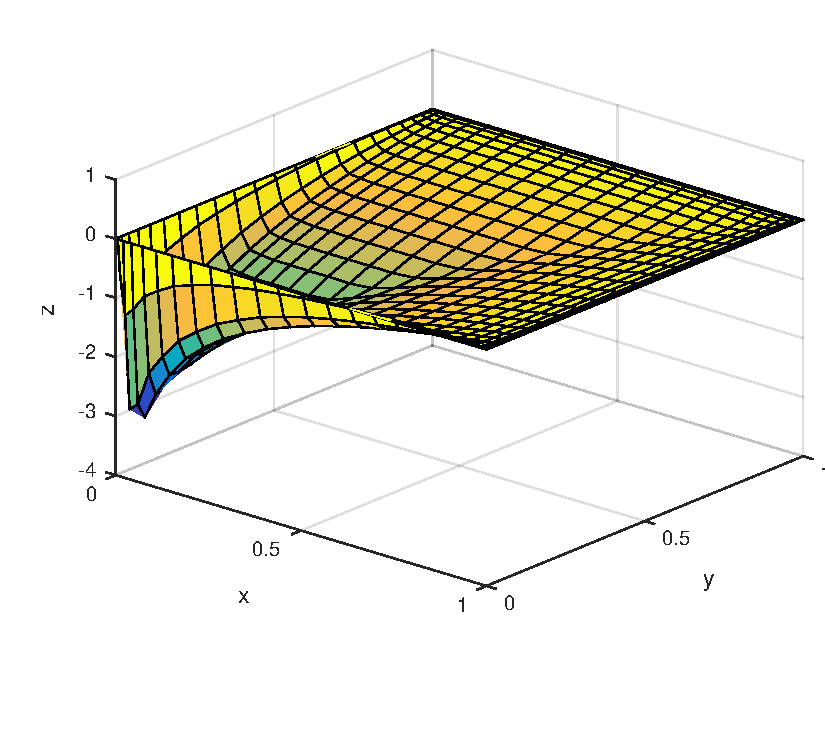
\includegraphics[width=\textwidth]{Figures/SpecLS_difftrans_aPos.pdf}
  %\end{subfigure}
  \begin{subfigure}[b]{0.48\textwidth}
	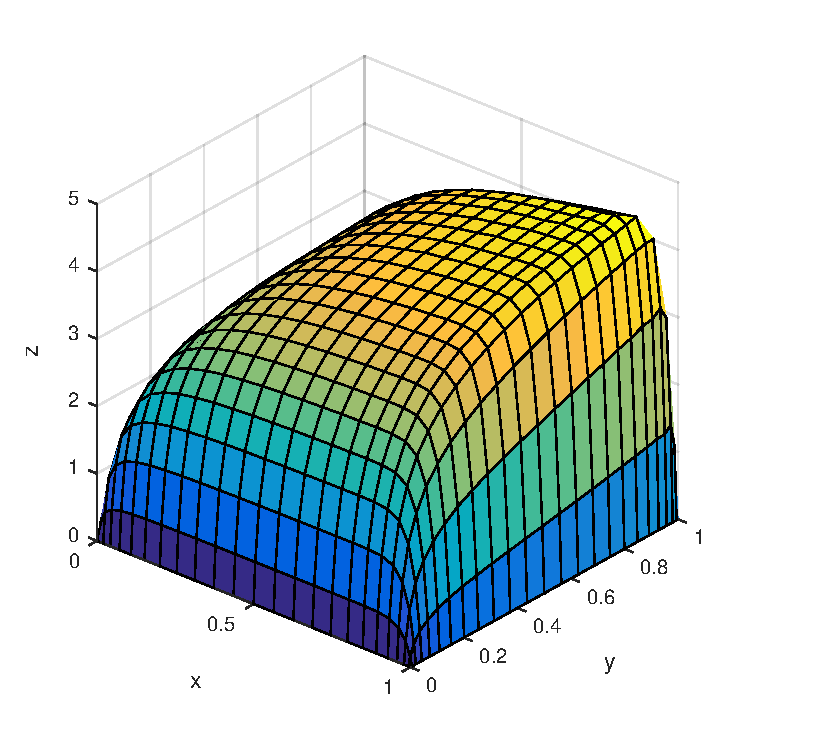
\includegraphics[width=\textwidth]{Figures/SpecGLS_difftrans_aPos.pdf}
  \end{subfigure}
          %(or a blank line to force the subfigure onto a new line)
  \vspace{-0.1\baselineskip}
  \caption{Surf plot of the numerical solution obtained from spectral methods of the diffusion transport problem solved by Galerkin to the left and with a combined GLS method to the right, with smoothening factor $\delta = 0.05$, both plots use the same parameters $\mu = 10^{-4}, N=25,\mathbf{b} = [x,y]$.}
  \label{fig:SurfDiffTransPositive}
\end{figure}
%
%
\begin{figure}[h]
  \centering
  \begin{subfigure}[b]{0.48\textwidth}
	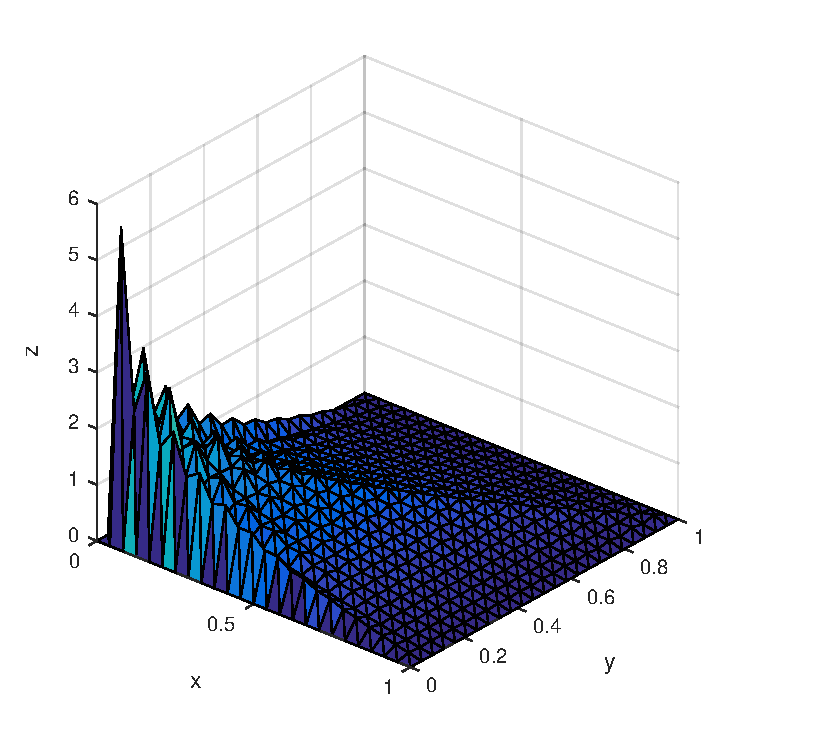
\includegraphics[width=\textwidth]{Figures/FEM_difftrans_aNeg.pdf}
  \end{subfigure}%
  \quad
  %\begin{subfigure}[b]{0.48\textwidth}
	%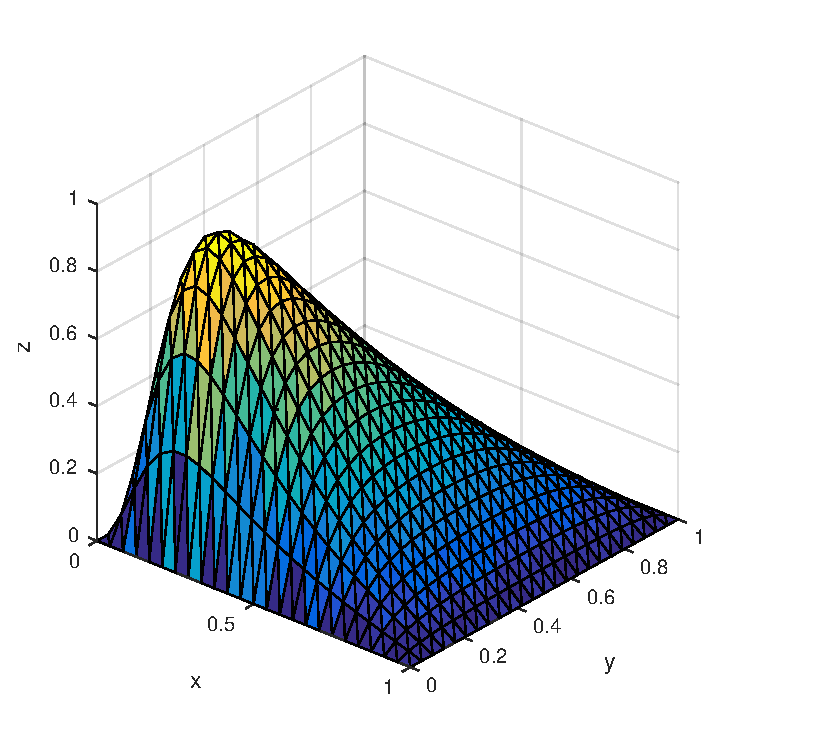
\includegraphics[width=\textwidth]{Figures/LSFEM_difftrans_aNeg.pdf}
  %\end{subfigure}
  \begin{subfigure}[b]{0.48\textwidth}
	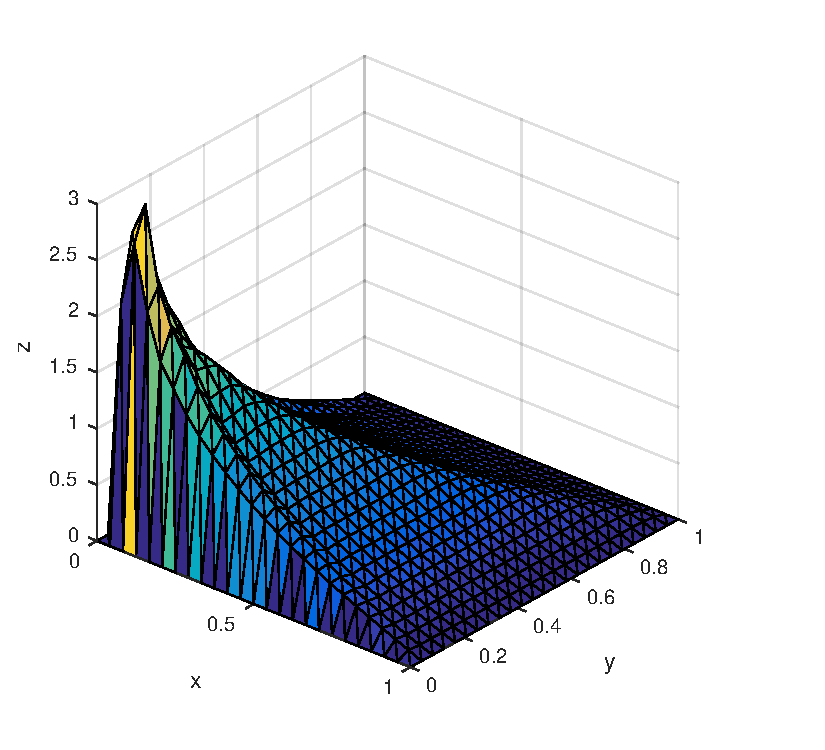
\includegraphics[width=\textwidth]{Figures/GLSFEM_difftrans_aNeg.pdf}
  \end{subfigure}
          %(or a blank line to force the subfigure onto a new line)
  \vspace{-0.1\baselineskip}
	\caption{Surf plot of the numerical solution of the diffusion transport problem solved by Galerkin FEM to the left and the combined GLS method to the right, with smoothening factor $\delta = 0.05$, both plots use the same parameters, $\mu = 10^{-4},N=25,\mathbf{b} = -[x,y]$.}
  \label{fig:SurfDiffTransPositiveFEM}
\end{figure}

%
%\begin{figure}[h!]
  %\centering
  %\begin{subfigure}[b]{0.48\textwidth}
	%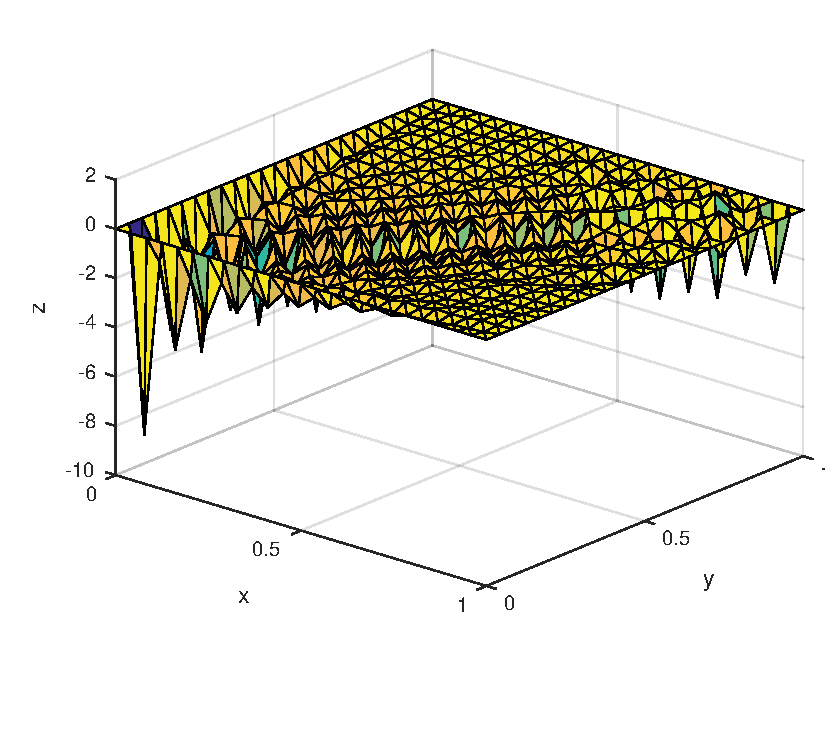
\includegraphics[width=\textwidth]{Figures/FEM_difftrans_aPos.pdf}
  %\end{subfigure}%
  %\quad
  %\begin{subfigure}[b]{0.48\textwidth}
	%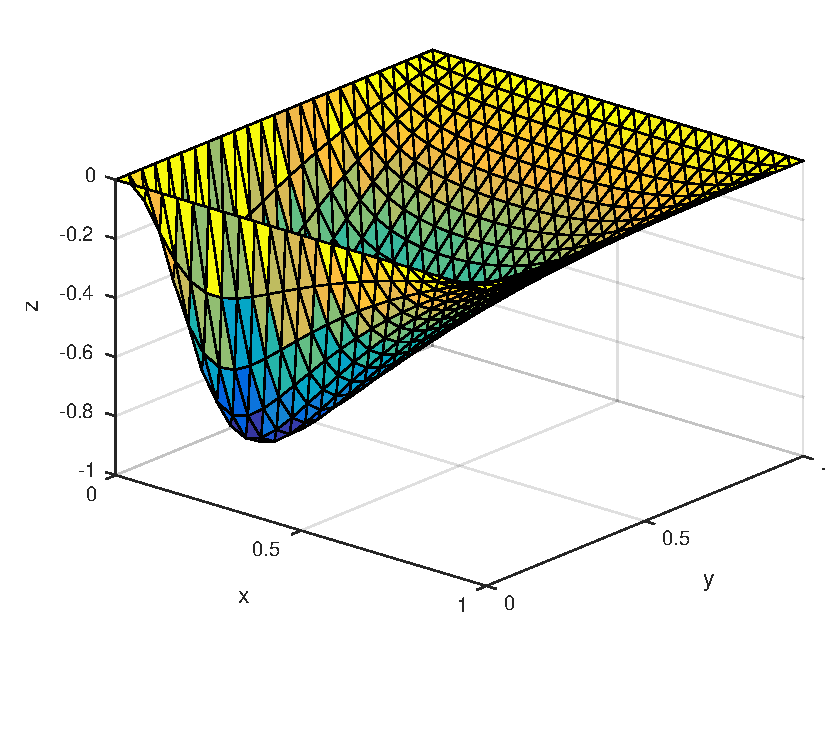
\includegraphics[width=\textwidth]{Figures/LSFEM_difftrans_aPos.pdf}
  %\end{subfigure}
  %\begin{subfigure}[b]{0.48\textwidth}
	%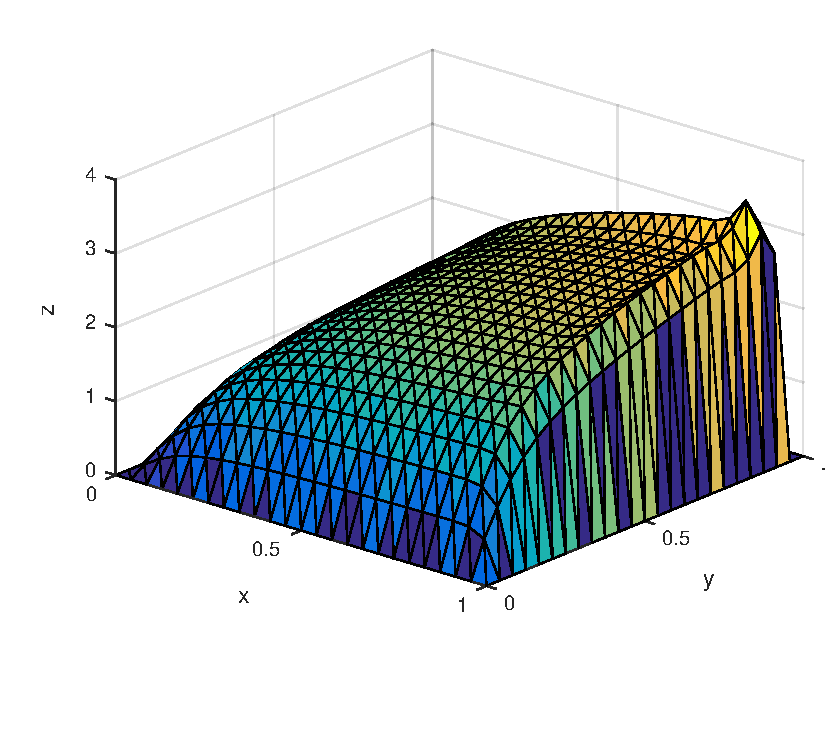
\includegraphics[width=\textwidth]{Figures/GLSFEM_difftrans_aPos.pdf}
  %\end{subfigure}
          %%(or a blank line to force the subfigure onto a new line)
  %\vspace{-0.1\baselineskip}
  %\caption{Surf plot of the numerical solution of the diffusion transport problem solved by Galerkin FEM to the left ,least-squares to the right and the combined GLS method below with $\delta = 0.05$, all the plots use the same parameters $\mu = 10^{-4}, N=25,\mathbf{b} = [x,y]$.}
  %\label{fig:SurfDiffTransPositiveFEM}
%\end{figure}
%\begin{figure}[hl]
	%\centering
  %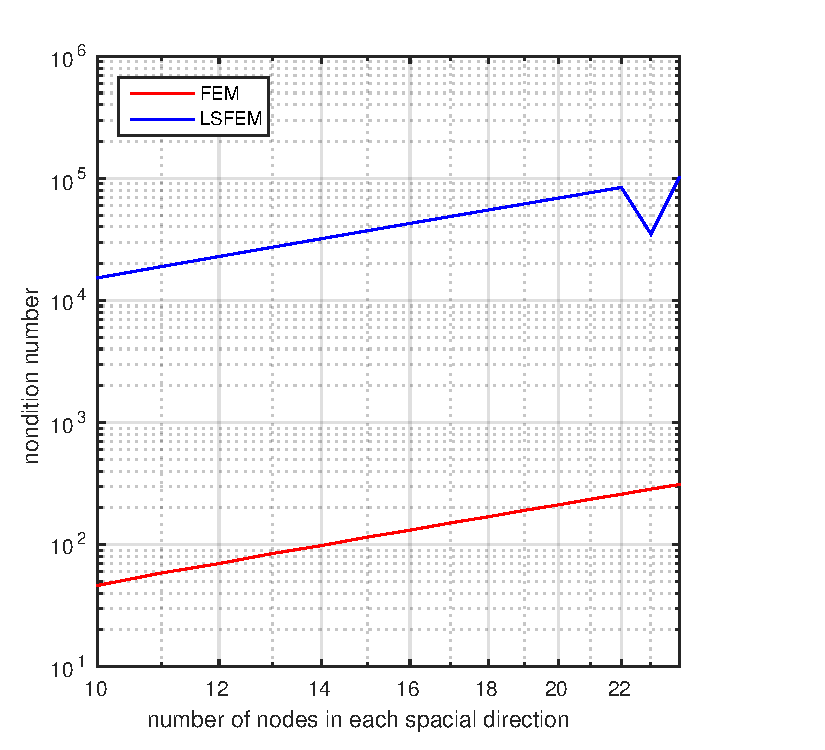
\includegraphics[width=80mm]{Figures/condFEM-LSFEM.pdf}
	%\caption{condition number of LSFEM and FEM}
	%\label{fig:conditionFEM}
%\end{figure}
%%
%%
%\begin{figure}[hl]
	%\centering
	%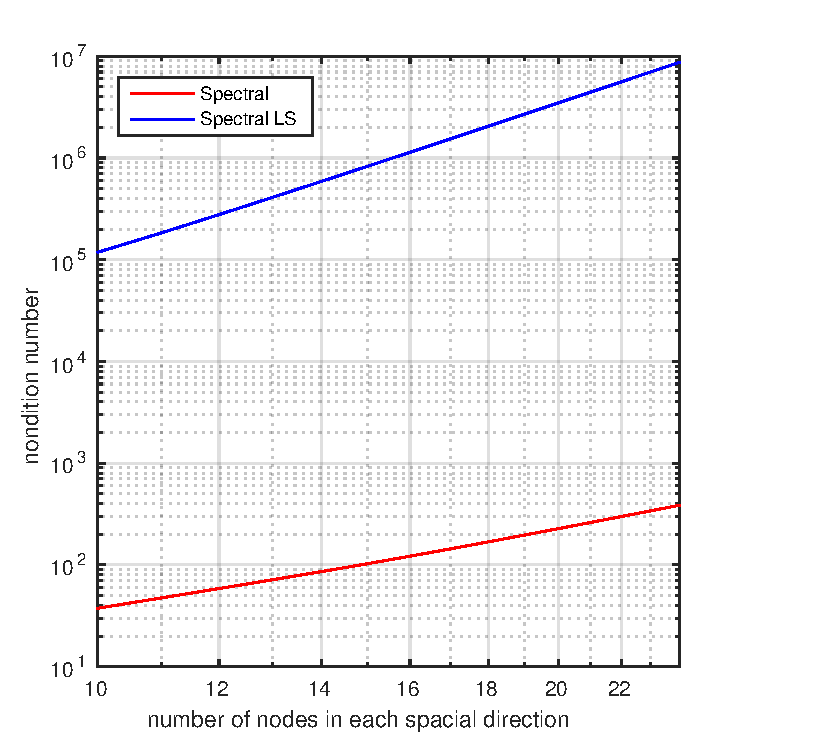
\includegraphics[width=80mm]{Figures/condSpec-SpecLS.pdf}
	%\caption{condition number of Spectral and LS-Spectral method}
	%\label{fig:conditionSpec}
%\end{figure}
%%

\subsection{Nonlinear results}

\begin{figure}[h]
  \centering
  \begin{subfigure}[b]{0.48\textwidth}
	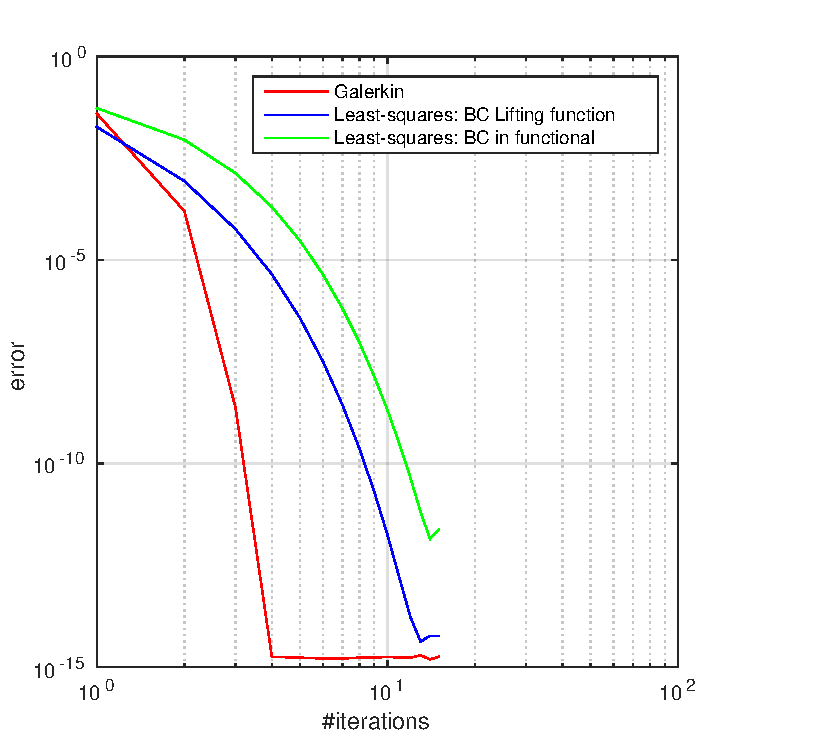
\includegraphics[width=\textwidth]{Figures/Spec_Nonlin_Convergence_Jnum.pdf}
  \end{subfigure}%
  \quad
  \begin{subfigure}[b]{0.48\textwidth}
	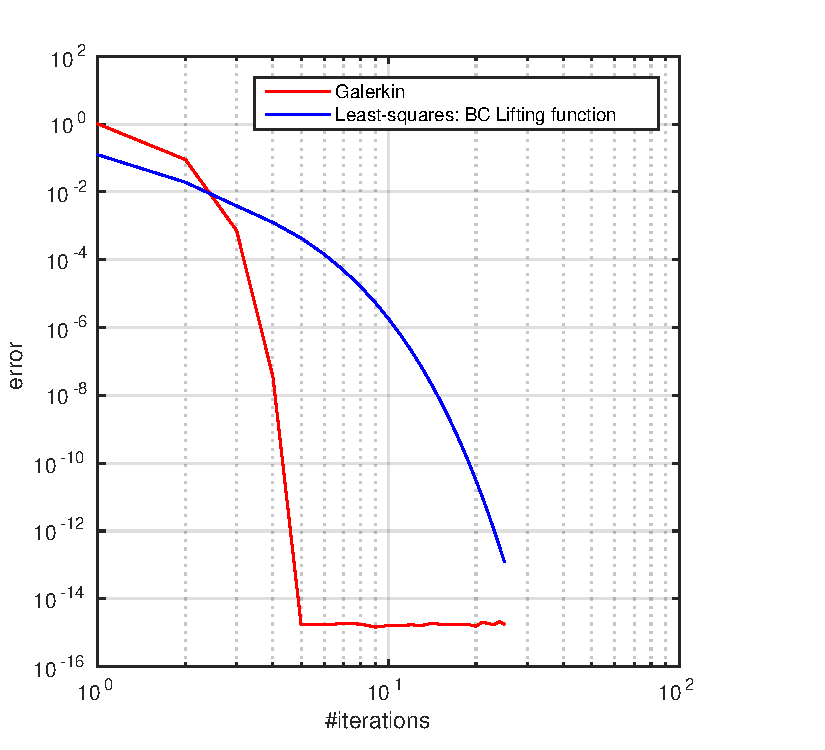
\includegraphics[width=\textwidth]{Figures/Spec_Nonlin_Convergence.pdf}
  \end{subfigure}%
  \vspace{-0.1\baselineskip}
	\caption{Convergence plot of the numerical solution of the nonlinear diffusion transport equation solved by spectral methods, In the figure to the left a numerical jacobian has been calculated and in the figure to the right the analytical one is used. $\mu = 1,N=15,\mathbf{b} = -[x^2,y^2]$.}
  \label{fig:SurfDiffTransPositiveFEM}
\end{figure}
